% Should be <2 pages

% **Problems**

% **Needs to contain**
% - Hardware Description on a more detailed level

% **Structure**

% - Hardware section
%     - Overview
%     - Decisions
% - Software section
%     - Overview
%     - Decisions

\section{Hardware Implementation}

% Overview
A similar paper conducted at the Royal Institute of Technology (KTH) earlier this year served as the main baseline for how the hardware was to be setup.\cite{hospital} The main components are the microcontroller, the scale as well as the ADC (Analog-to-Digital Converter). Apart from this, an adequate power source is needed to provide energy to all components. 

% Decisions
\subsection{Scale}
The scale used for this paper is a Tedea Huntleigh - Model 1022. It is a small and simple model, and the specific device used in this paper had a maximum capacity of 50 kg.\cite{load-cell-data} In figure \ref{fig:load_cell_wiring} we can see the labels of the four wires needed to hook up the load cell. The \textit{Input+} and \textit{Input-} signify the voltage input and ground. \cite{load-cell-spec} \textit{Output+} and \textit{Output-} will output a positive respectively a negative charge of about 1.5 voltage . During weighing, the internal resistance in the load cell will change ever so slightly, and the two outputs will have a small difference in the millivoltage range. This difference represents the weight measurement, and can be translated to a corresponding kg/lb value. In general, the more voltage the scale is supplied with, the greater this millivoltage range can be, which (in theory) means larger accuracy when weighing. No two load cells are the same, and they need to be calibrated to output the correct kg/lb value.

\begin{figure}[h]
	\centering
	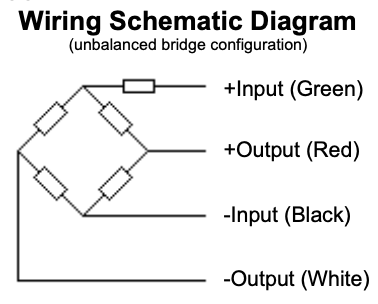
\includegraphics[width=0.3\textwidth]{load-cell-wiring.png}
	\caption{The wiring schematic for the load cell}
	\label{fig:load_cell_wiring}
\end{figure}


\subsection{ADC}
To convert the millivoltage output from the load cell into a digital signal, an ADC is needed. The device used in this paper is an HX711, and apart from being a converter, it also serves as an amplifier for the load cell signal. The front of the ADC is visible in the top of figure \ref{fig:hx711}, with the backside below, where the pinout of all the wires from the load cell should be connected. The color coding of the wiring is not the same for all load cells, and the backside should be checked so that the connections follow the correct wiring schematic. 

The ADC outputs data via two of its pins, the DAT and the CLK. The CLK pin will output 0 if it is ready to send data, and 1 if it is not ready. When it is ready, the DAT pin will send  a series of 0s and 1s that can be converted from binary to a decimal value, which will then represent the output of the load scale.\cite{hx711-datasheet} Multiple code libraries have been written to handle this for the user, and which only require a specification of which pins are being used by CLK and DAT respectively. For this paper, a library written for micropython was used.\cite{hx711-lopy}

\begin{figure}[h]
	\centering
	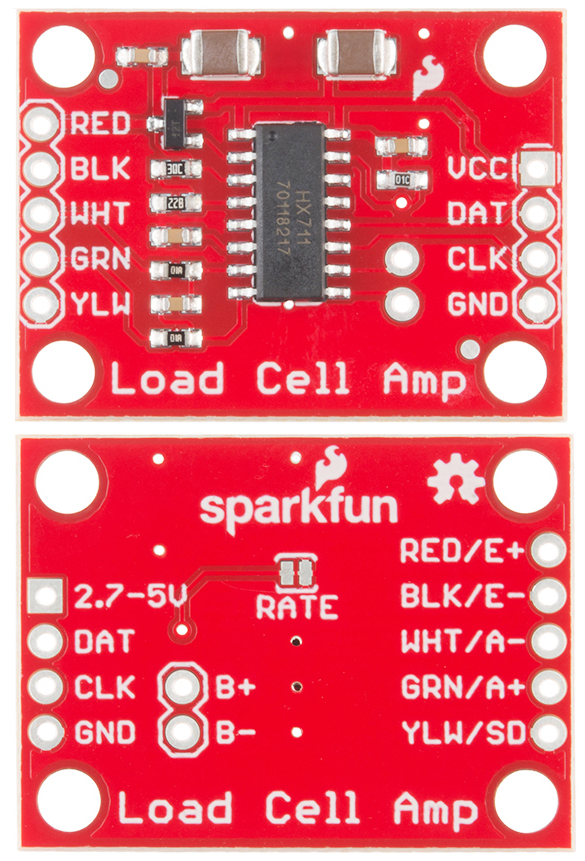
\includegraphics[width=0.3\textwidth]{hx711.png}
	\caption{The front and back of the HX711.}
	\label{fig:hx711}
\end{figure}

\begin{figure}[h]
	\centering
	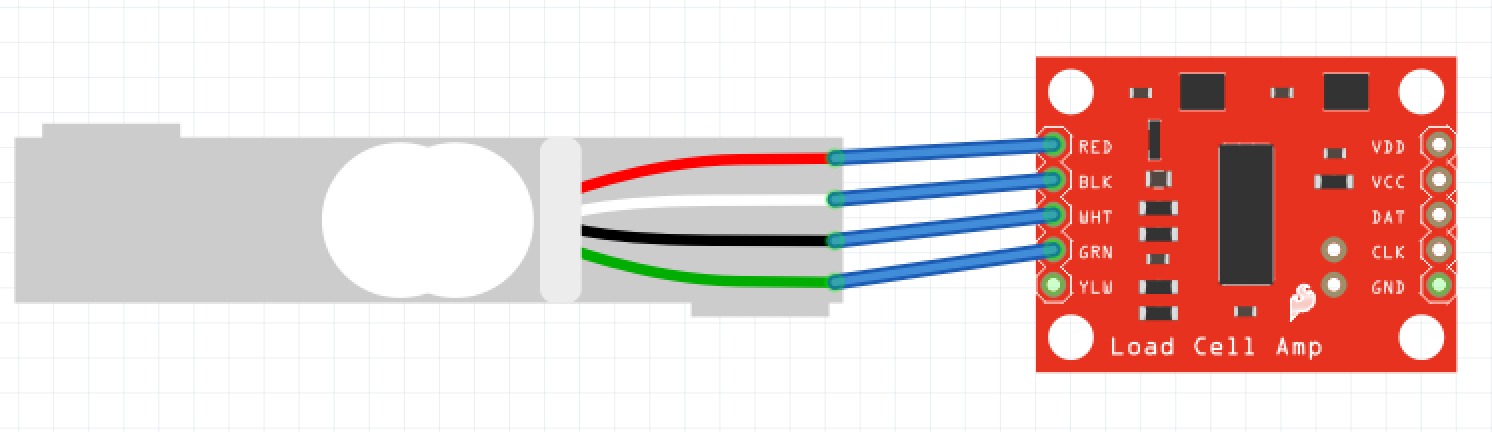
\includegraphics[width=0.6\textwidth]{load-cell_hx711.png}
	\caption{The load cell wired to the ADC. The color of the wiring schema corresponds to the schematic seen in figure. \ref{fig:load_cell_wiring}}
	\label{fig:load_cell_hx711}
\end{figure}

\subsection{Microcontroller}
The microcontroller used for this paper is the FiPy development board from PyCom. It boasts a wide range of capabilities when it comes to communication protocols, NB-IoT being one of the five available.\cite{fipy-docs} With the supplied expansion board, connections via pinout is possible. It runs on micropython, which is an implementation of Python 3 optimized to run on microcontrollers.\cite{micropython} The FiPy can be seen on figure \ref{fig:fipySide} and its expansion board on figure \ref{fig:exp_board}
\begin{figure}[H]
\begin{subfigure}{0.5\textwidth}
	\centering
	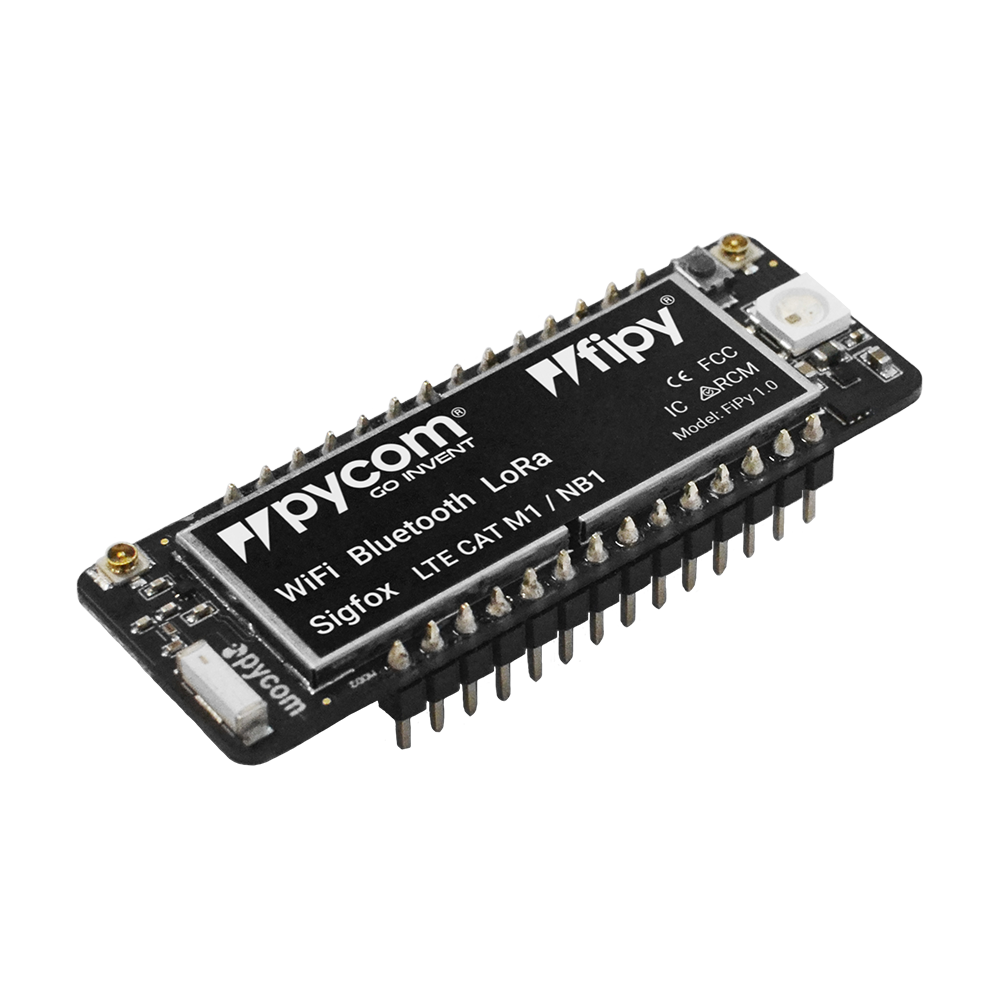
\includegraphics[width=0.8\textwidth]{fipySide.png}
	\caption{The FiPy as seen from the side}
	\label{fig:fipySide}
\end{subfigure}
%
\begin{subfigure}{0.5\textwidth}
	\centering
	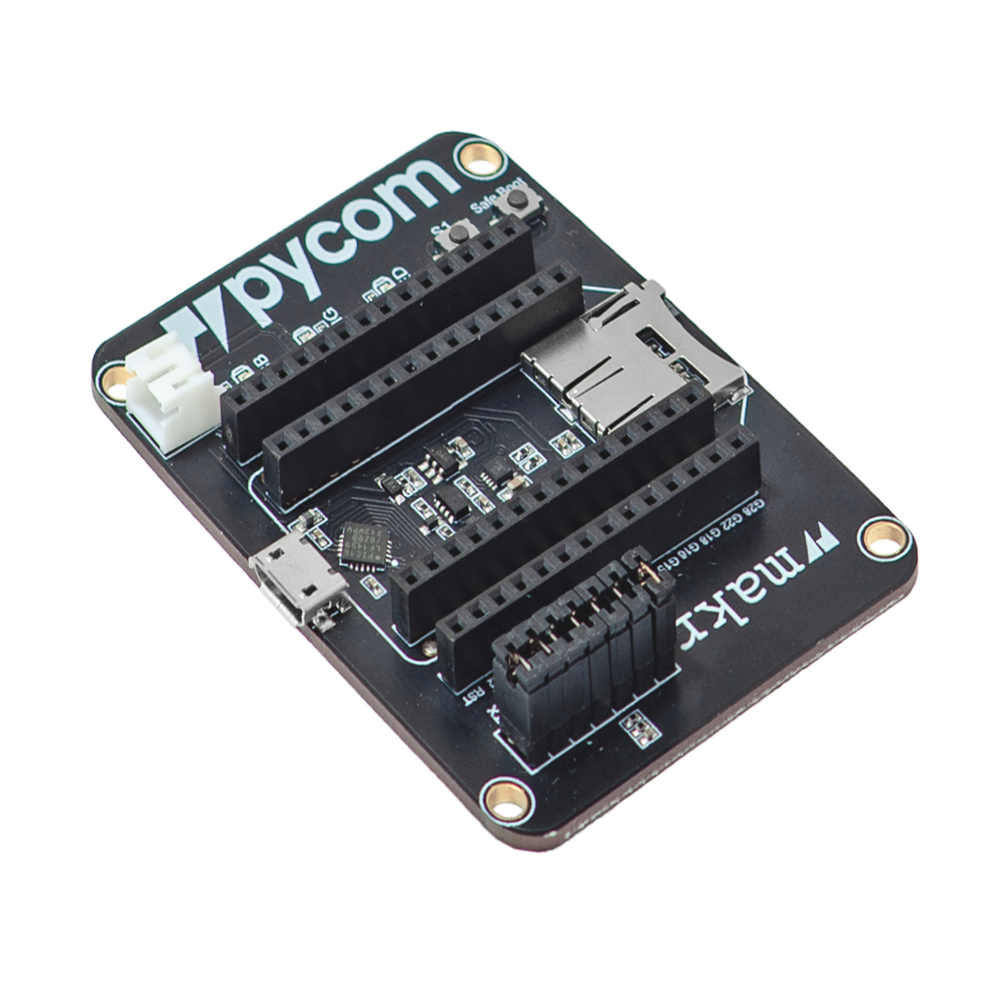
\includegraphics[width=0.8\textwidth]{exp_board.png}
	\caption{The expansion board of the FiPy}
	\label{fig:exp_board}
\end{subfigure}
\caption{The Fipy and the expansion board 3.0}
\end{figure}

\subsection{Powering the Project}
In the early stages of the project, the hardware was powered via USB cable from a computer. Since the USB was of type micro, the voltage output was 5V. Since this did not yield a functional behavior from the components, another setup was tried.
\begin{figure}[h]
	\centering
	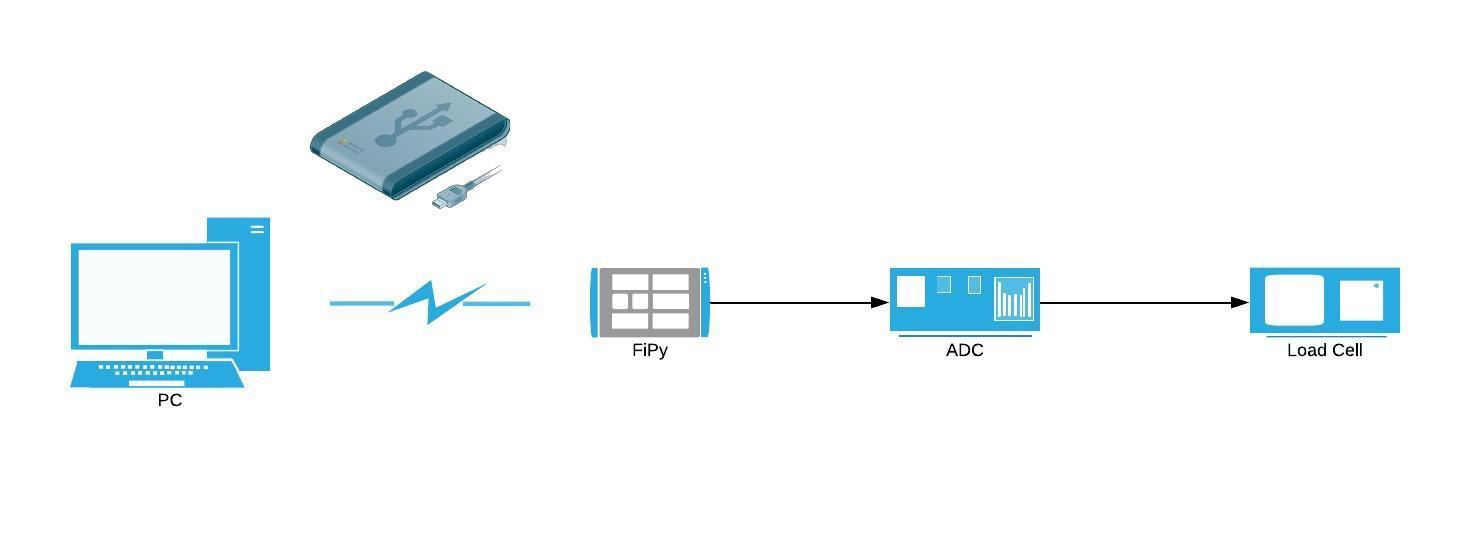
\includegraphics[width=0.8\textwidth]{wiring_comp.jpeg}
	\caption{The first wiring used\cite{lucid-chart}}
	\label{fig:wiring_comp}
\end{figure}

The second approach used two different power, where the ADC was powered by a wall outlet at a higher voltage, while the FiPy kept the USB. Once again, this did not produce a valid result.
\begin{figure}[H]
	\centering
	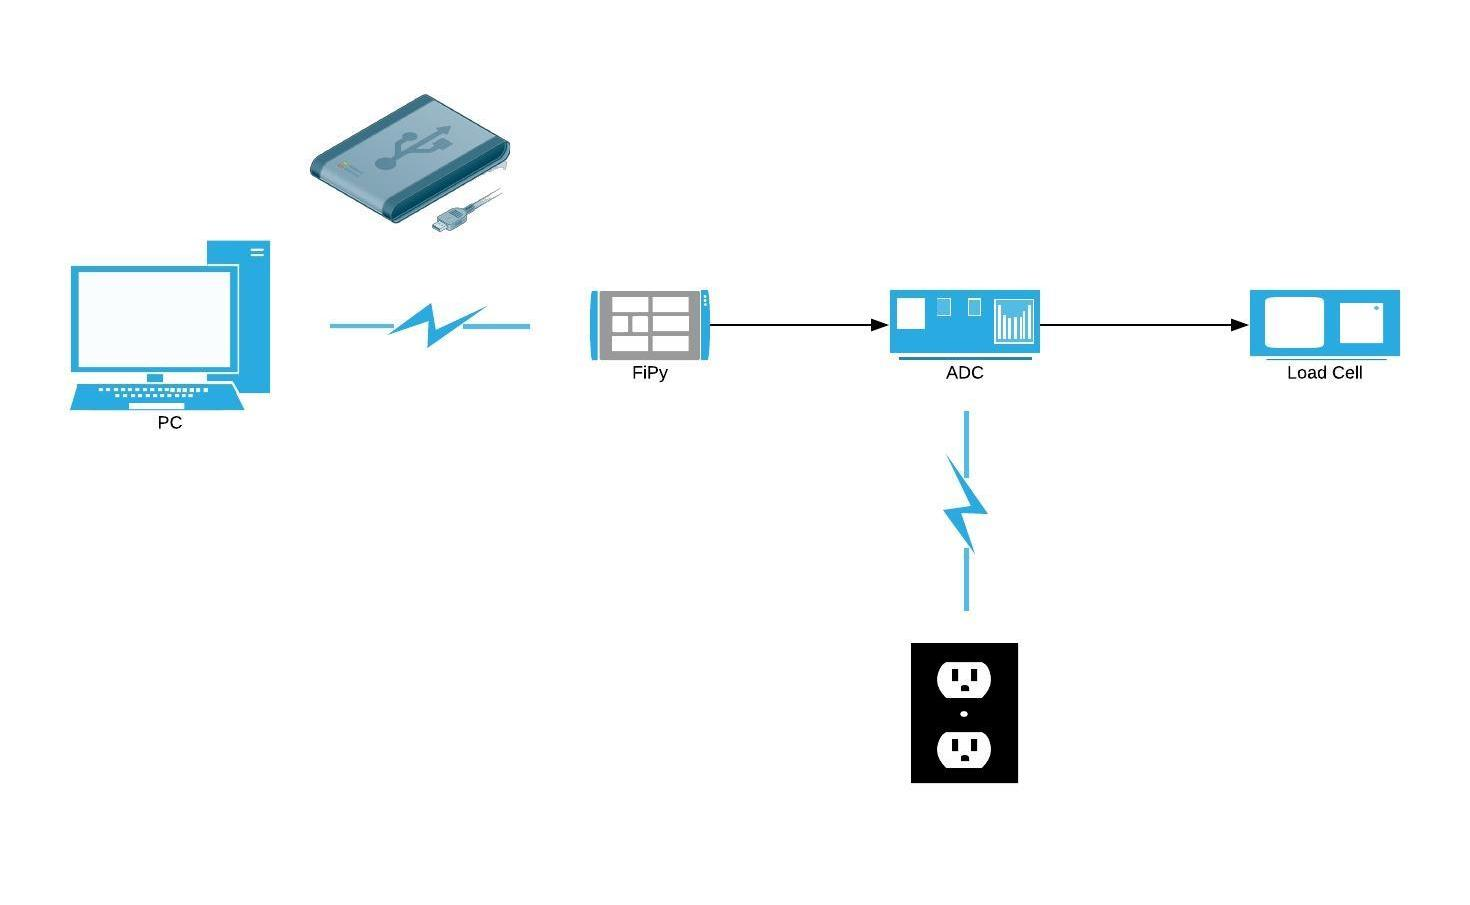
\includegraphics[width=0.8\textwidth]{wiring_outlet.jpeg}
	\caption{The second wiring used\cite{lucid-chart}}
	\label{fig:wiring_outlet}
\end{figure}

The final wiring involved an Otii battery toolbox, which is an advanced piece of hardware used to profile and emulate batteries.\cite{otii-web} With this piece of equipment, a common ground was provided to all components, as well as adequate voltage. It was capable of supplying 5V to both the FiPy and the ADC at the same time, which in turn enabled stable output of data values. 
\begin{figure}[H]
	\centering
	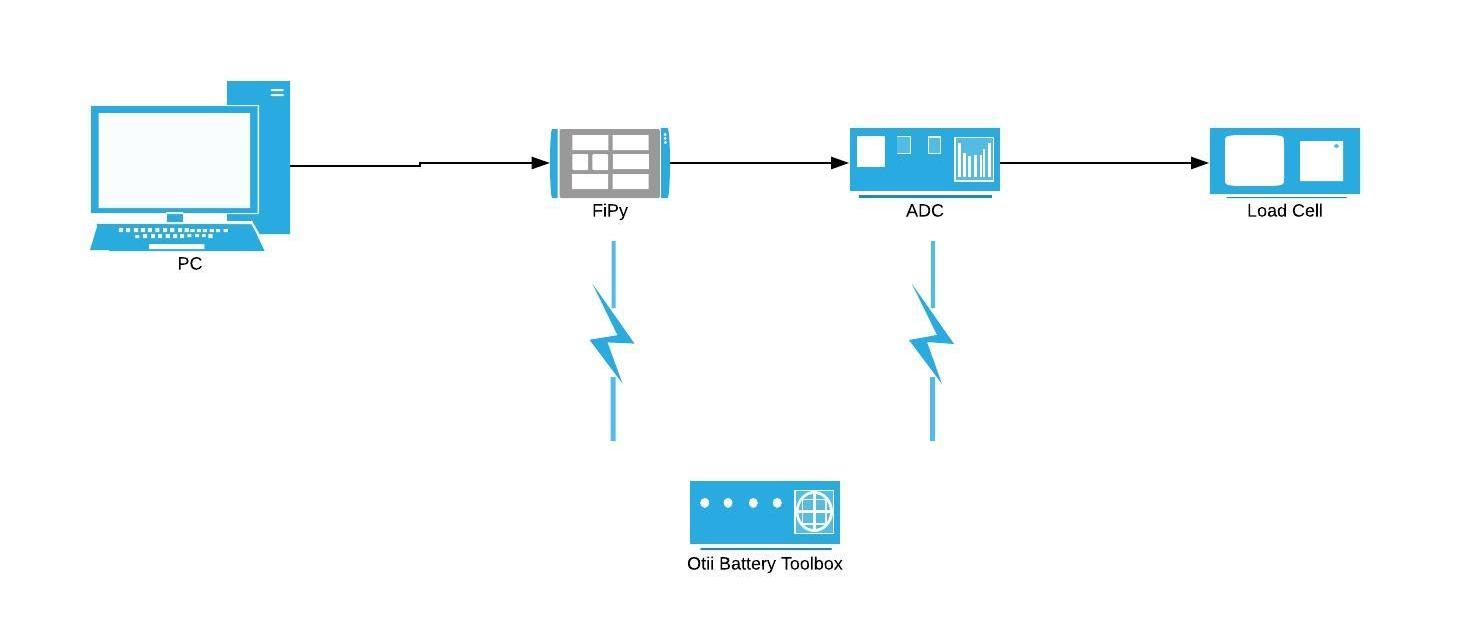
\includegraphics[width=0.8\textwidth]{wiring_otii.jpeg}
	\caption{The third wiring used\cite{lucid-chart}}
	\label{fig:wiring_otii}
\end{figure}

All data values produced by the load cell and ADC during these tests were raw values, as a calibration for kg/lb values for our intents and purposes would not bring any significant enhancements to the project.

\section{Software Implementation}
The FiPy code runs on MicroPython, an implementation of Python 3 optimized for microcontrollers. MicroPython only executes two files on its system's root folder, the \lstinline{boot.py} and the \lstinline{main.py} files. Any remaining code must be placed in the \lstinline{/lib/} folder. The \lstinline{boot.py} runs first, and is intended to contain low-level code that is meant to configure the hardware. The \lstinline{main.py} file contains the main program loop, and imports auxiliary files from the \lstinline{/lib/} folder.
The two files used for the implementation in the \lstinline{/lib/} folder are \lstinline{reader.py} and \lstinline{error_tracker.py}. A test file has been written for each module, to ensure that the software did not regress during development. All python classes and their respective tests can be found in the appendix. 

The software tests were built using a micropython library called \lstinline{unittest}, and the tests were constructed so that they would mirror the requirements set in the Requirements chapter. The files used for testing in the \lstinline{/lib/} folder are the \lstinline{unittest.py}, \lstinline{test_reader_poll_rate.py} and \lstinline{test_error_tracker.py}.